\noindent
Dado que el objetivo del proyecto es comparar tres diferentes métodos 
de súper resolución, en esta sección se presentarán las actividades
requeridas para la implementación de los métodos. Considerando desde los 
requisitos de software, hardware y datos de entrenamiento en caso sean 
necesarios. 

\subsection{Example-Based Super-Resolution}
\subsubsection{Construcción de diccionario}
\noindent
Para el primero de ellos, se retoma la literatura expuesta en \cite{freeman}
comenzando con la generación del diccionario donde se encuentran relacionados 
los parches de baja y alta resolución. Previo a esto, es necesario pre-procesar
el conjunto de imágenes para su posterior segmentación. 

De acuerdo a las indicaciones, se deben tener pares de imágenes en alta y baja 
resolución. Para esta implementación se ha considerado las primeras 14 imágenes
de \cite{MIRFLICKR} las cuales están en alta resolución. En la Figura \ref{fig:fr_dataset}
puede observarse que el conjunto de imágenes no guardan una relación en específico
por lo que los requisitos para aplicar el algoritmo son bastante flexibles.

\begin{figure}[H]
    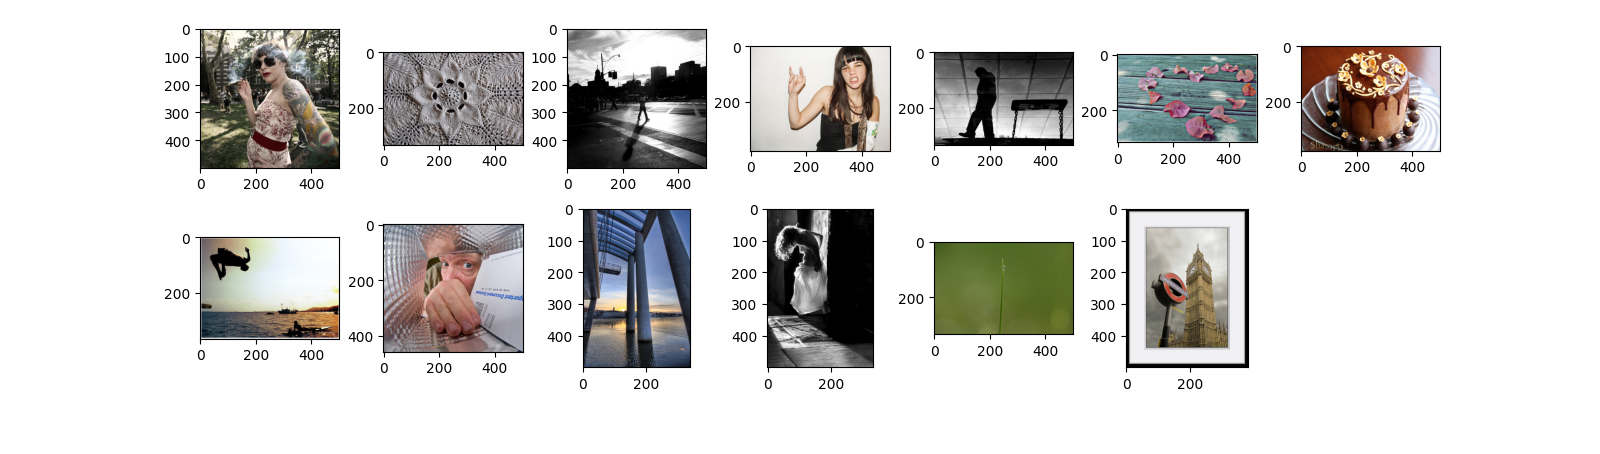
\includegraphics[scale = 0.4]{ fr_dataset.png }
    \centering
    \caption{ \emph{Dataset} utilizado para construcción de diccionario}
    \label{fig:fr_dataset}
\end{figure}

En la Figura \ref{fig:fr_interpolacion} se presenta el procedimiento realizado para
construir el conjunto de imágenes de baja resolución mediante una reducción por el 
factor $\frac{1}{\Omega}$ y posterior escalado de $\Omega$ con el objetivo de 
perder información al escalar la imagen una vez realizada la compresión, forzando
la baja resolución. Para esta implementación se consideró un factor $\Omega = 4$. 

\begin{figure}[H]
    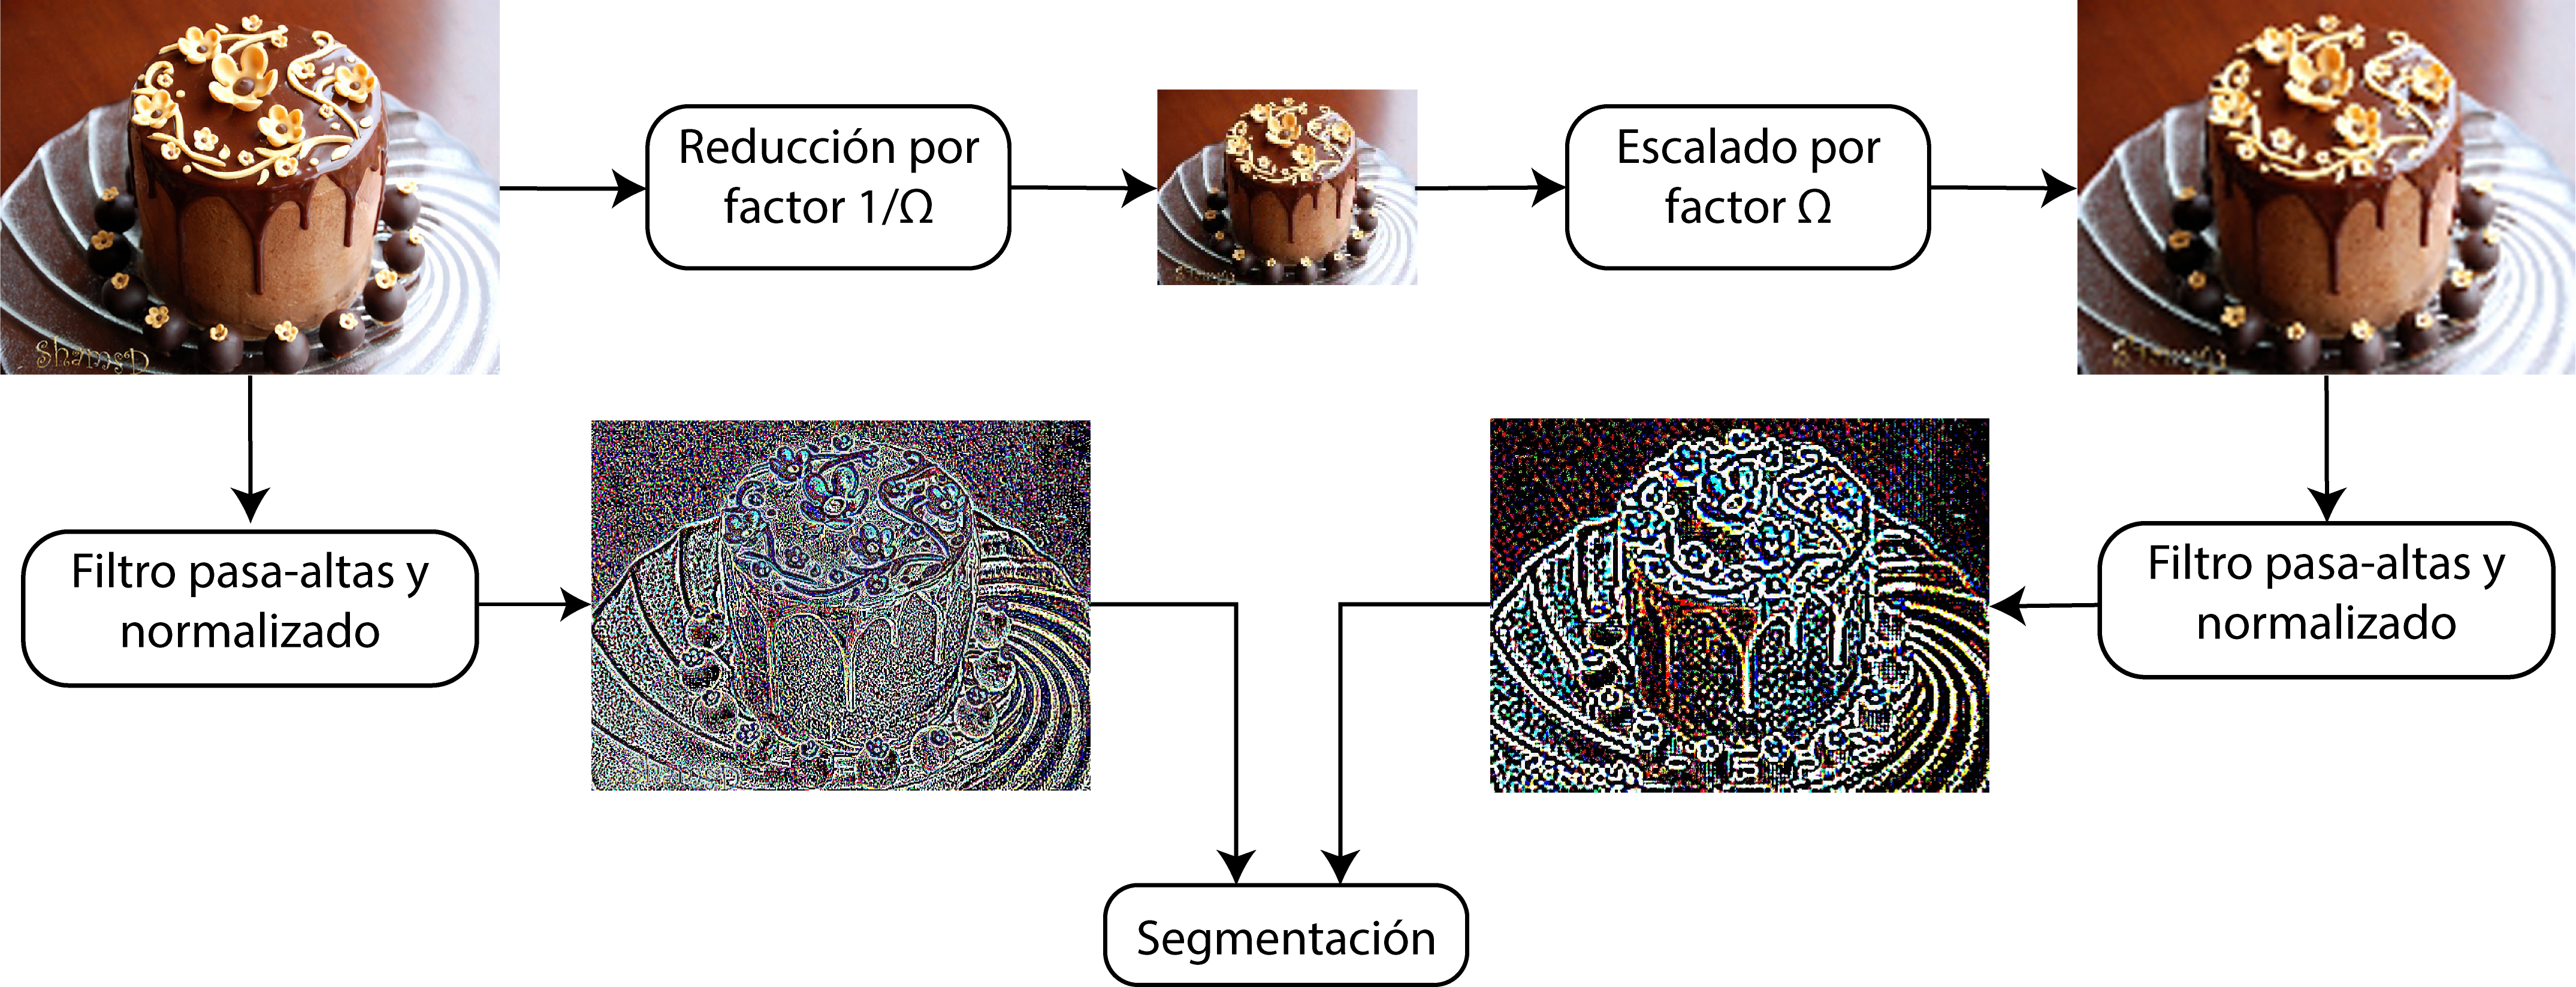
\includegraphics[scale = 0.6]{ fr_prepdic.png }
    \centering
    \caption{Preparación de base de entrenamiento mediante algoritmos de interpolación}
    \label{fig:fr_interpolacion}
\end{figure}

Como se presenta en la Figura \ref{fig:fr_interpolacion}, ambas imágenes 
rquieren ser filtradas (para reducir la cantidad de información innecesaria)
y normalizadas (con el objetivo de generalizar el algoritmo) para realizar el
proceso de segmentación. Para cada imagen filtrada $\text{img}?f$ se utilizó la función de\
\emph{OpenCV} \emph{GaussianBlur} considerando una desviación estándar $\sigma = 1$
con el fin de restar la imagen desenfocada (frecuencias medias y bajas) a la imagen 
original para dejar sólo las frecuencias altas (detalles) tal como se presenta
en la expresión \eqref{eqn:filtroPH}.

\begin{align}
    \label{eqn:filtroPH}
    \text{img}_f = \text{img} - \text{\emph{cv2.GaussianBlur(img, }(0,0),}\, \sigma)
\end{align}

Para obtener la imagen normalizada $\text{img}_n$ se consideró la expresión \eqref{eqn:normalizado}.

\begin{align}
    \label{eqn:normalizado}
    \text{img}_n = \frac{\text{img}_f-\text{min}(\text{img}_f)}{\text{max}(\text{img}_f)-\text{min}(\text{img}_f)}\cdot 255
\end{align}

De esta manera, el \emph{segmentador} puede realizar un barrido bidimensional (de acuerdo a 
la Figura \ref{fig:fr_dic}) en cada imagen 
con el objetivo de recolectar los parches en alta y baja resolución con 
dimensiones de $5x5$ y $7x7$ respectivamente.

\begin{figure}[H]
    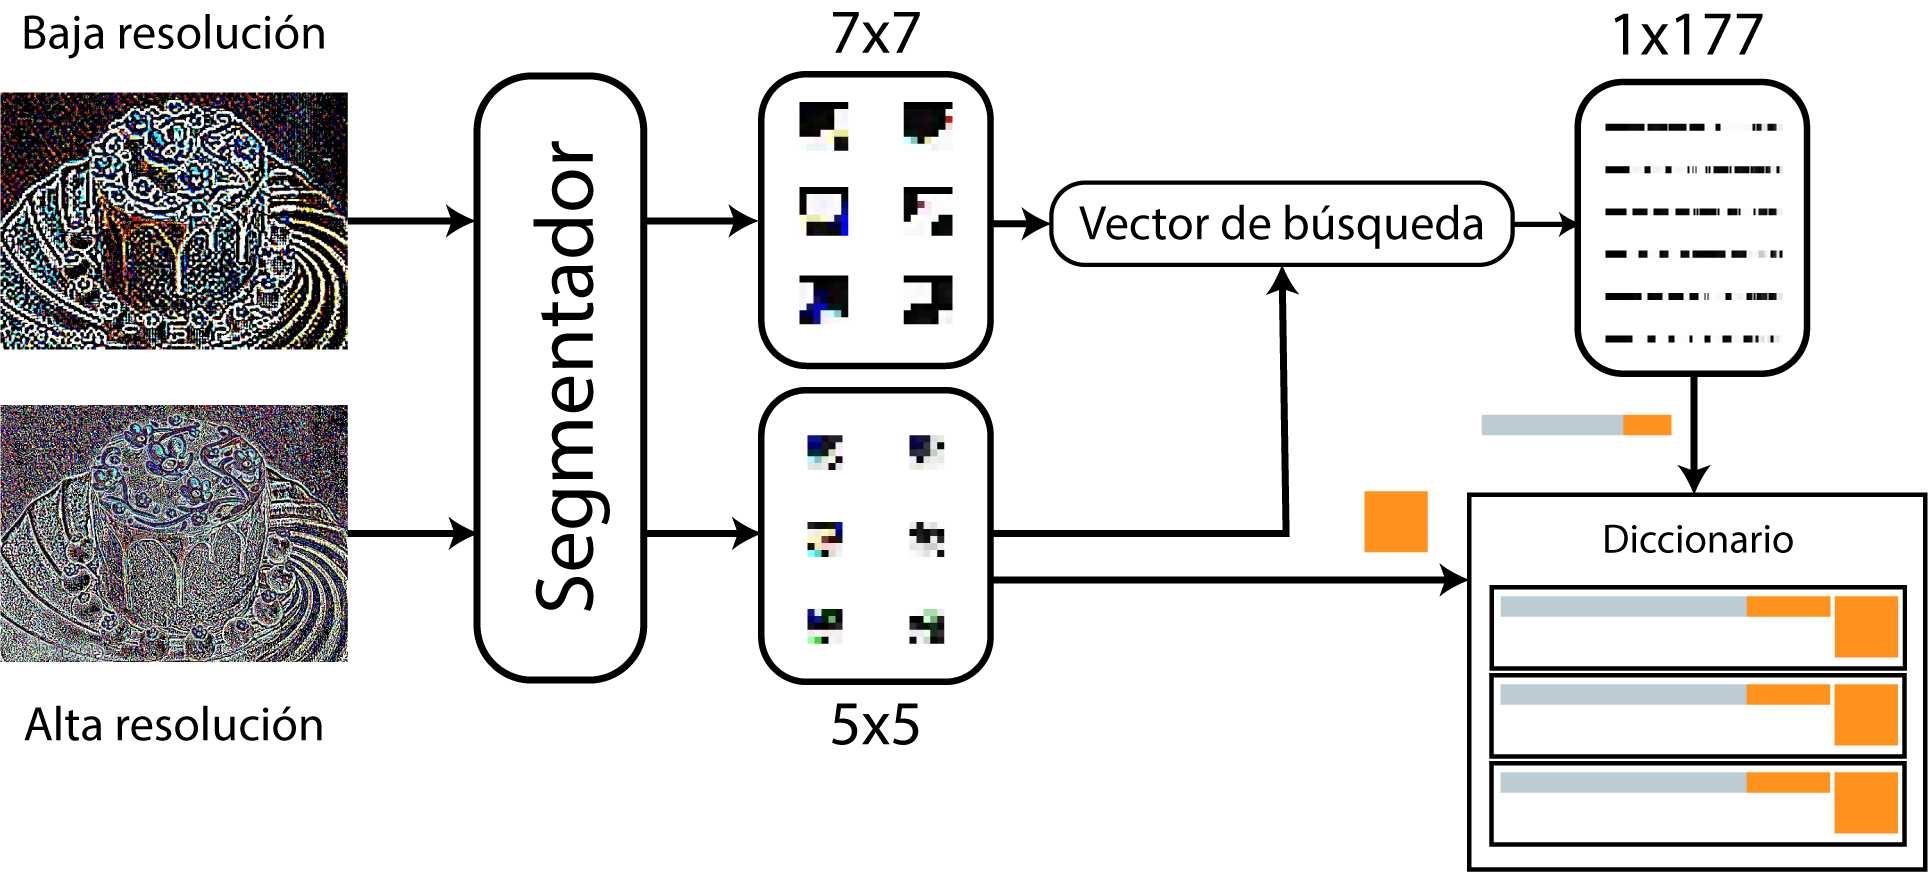
\includegraphics[scale = 1.2]{ fr_segmentado.png }
    \centering
    \caption{ Segmentación y almacenamiento de parches en diccionario }
    \label{fig:fr_segmentador}
\end{figure}

Posteriormente, el parche de baja resolución es reordenado para formar un 
vector fila en $\mathbb{R}^{1\times147}$ para concatenarse con el vector de superposición
(en $\mathbb{R}^{1\times30})$ que considera la primera fila y primera columna del
parche de alta resolución. A dicha concatenación se le nombrará como 
\emph{vector de búsqueda}. En la Figura \ref{fig:fr_segmentador} puede observarse
al conjunto de vectores de búsqueda que serán guardados en el \emph{diccionario}
junto con los parches de alta resolución. 

El proceso anterior es realizado para cada imagen y dado que cada una es de 
dimensiones diferentes, el número de parches será distinto. Cabe 
destacar que el almacenamiento de los 154,125 vectores realizó
mediante el paquete \emph{h5py} en el archivo \emph{diccionario.h5},
ya que es recomendable para su implementación en algoritmos de búsqueda. 

\subsubsection{Algoritmo de búsqueda}
\noindent
Una vez construido el \emph{diccionario}, es necesario establecer el algoritmo de 
búsqueda para que cuando se realice la segmentación de la imagen a mejorar 
su resolución se busquen los parches de alta resolución de acuerdo al 
\emph{vector de búsqueda}.

Para esto, \cite{freeman} propone el uso de algoritmos de búsqueda como 
\emph{el vecino más cercano} para encontrar al vector más próximo a la solicitud
y con ello asociar al parche de alta resolución correspondiente. 

Utilizando la función \emph{NearestNeighbors} del paquete \emph{sklearn.neighbors} \cite{scikit-learn},
la implementación resulta sencilla una vez ordenados todos los vectores en el 
diccionario. 

Para verificar que el algoritmo funciona adecuadamente, se ha propuesto un 
parche externo de baja resolución (\emph{solicitud}) para 
que encuentre al parche de baja resolución más cercano que esté dentro del
\emph{diccionario} y asocie con el parche de alta resolución. En la Figura
\ref{fig:fr_vecinos} puede observarse que el primer pixel tiene un color 
diferente y aun así realiza la aproximación adecuadamente en 8.9 $s$
utilizando el algoritmo \emph{Ball Tree}.  

\begin{figure}[H]
    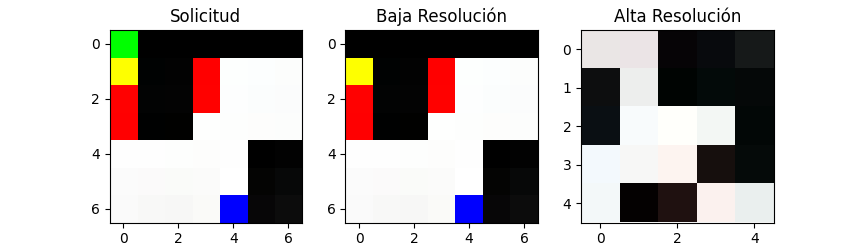
\includegraphics[scale = 0.6]{ fr_vecinos.png }
    \centering
    \caption{ Ejemplo de búsqueda de parches en diccionario}
    \label{fig:fr_vecinos}
\end{figure}

Respecto a la complejidad temporal de cada algoritmo, se presenta en 
la Tabla \ref{fig:fr_vecinos} otros algoritmos 
que de acuerdo a \cite{NN_search} cuenta la función utilizada.

\begin{table}[H]
    \caption{Tiempos de algoritmo de búsqueda}
    \label{tb:tiempos_snn}
    \centering
    \begin{tabular}{|c|c|}
    \hline
    \textbf{Algoritmo}    & \textbf{Tiempo} {[}s{]} \\ \hline
    Auto         & 9.8            \\ \hline
    Fuerza Bruta & 9.5            \\ \hline
    KD Tree      & 9.5            \\ \hline
    Ball Tree    & 8.9            \\ \hline
    \end{tabular}
\end{table}

Note que para fines de eficiencia considerando $D$ como dimensiones 
y $N$ como número de elementos, resulta más conviente el uso del algoritmo
\emph{Ball Tree} dado que complejidad es $\mathcal{O}[D\,\text{log}|N| ]$,
mientras que para el algoritmo de \emph{fuerza bruta} es
$\mathcal{O}[D\,\text{log}|N| ]$. Por otro lado, el algoritmo \emph{KD Tree}
tienen una complejidad $\mathcal{O}[D\,\text{log}|N| ]$ cuando $D$ es menor a 20
dimensiones. Sin embargo, si $D$ aumenta, entonces su complejidad resulta
$\mathcal{O}[D\,N]$. Por lo mismo, \emph{Ball Tree} es el algoritmo más rápido
para esta aplicación dados los resultados de la Tabla \ref{tb:tiempos_snn}. 

\subsubsection{Algoritmo de predicción}
\noindent
Teniendo ya el diccionario y el algoritmo de búsqueda, es posible aplicar el
\emph{algoritmo de un paso} propuesto por \cite{freeman} para mejorar la 
resolución de la imagen de entrada. Para ello nos basamos en el diagrama
presentado en la Figura \ref{fig:fr_algoritmo} realizando cada uno de los 
pasos mediante un paquete desarrollado por nosotros en Python. 

En la Figura \ref{fig:fr_proceso} puede observarse el proceso realizado para mejorar 
la resolución de la imagen ejemplo. Para este caso se ha considerado un escalado
con factor  $\Omega=2$ y factor de superposición de $\alpha=0.05$.

\begin{figure}[H]
    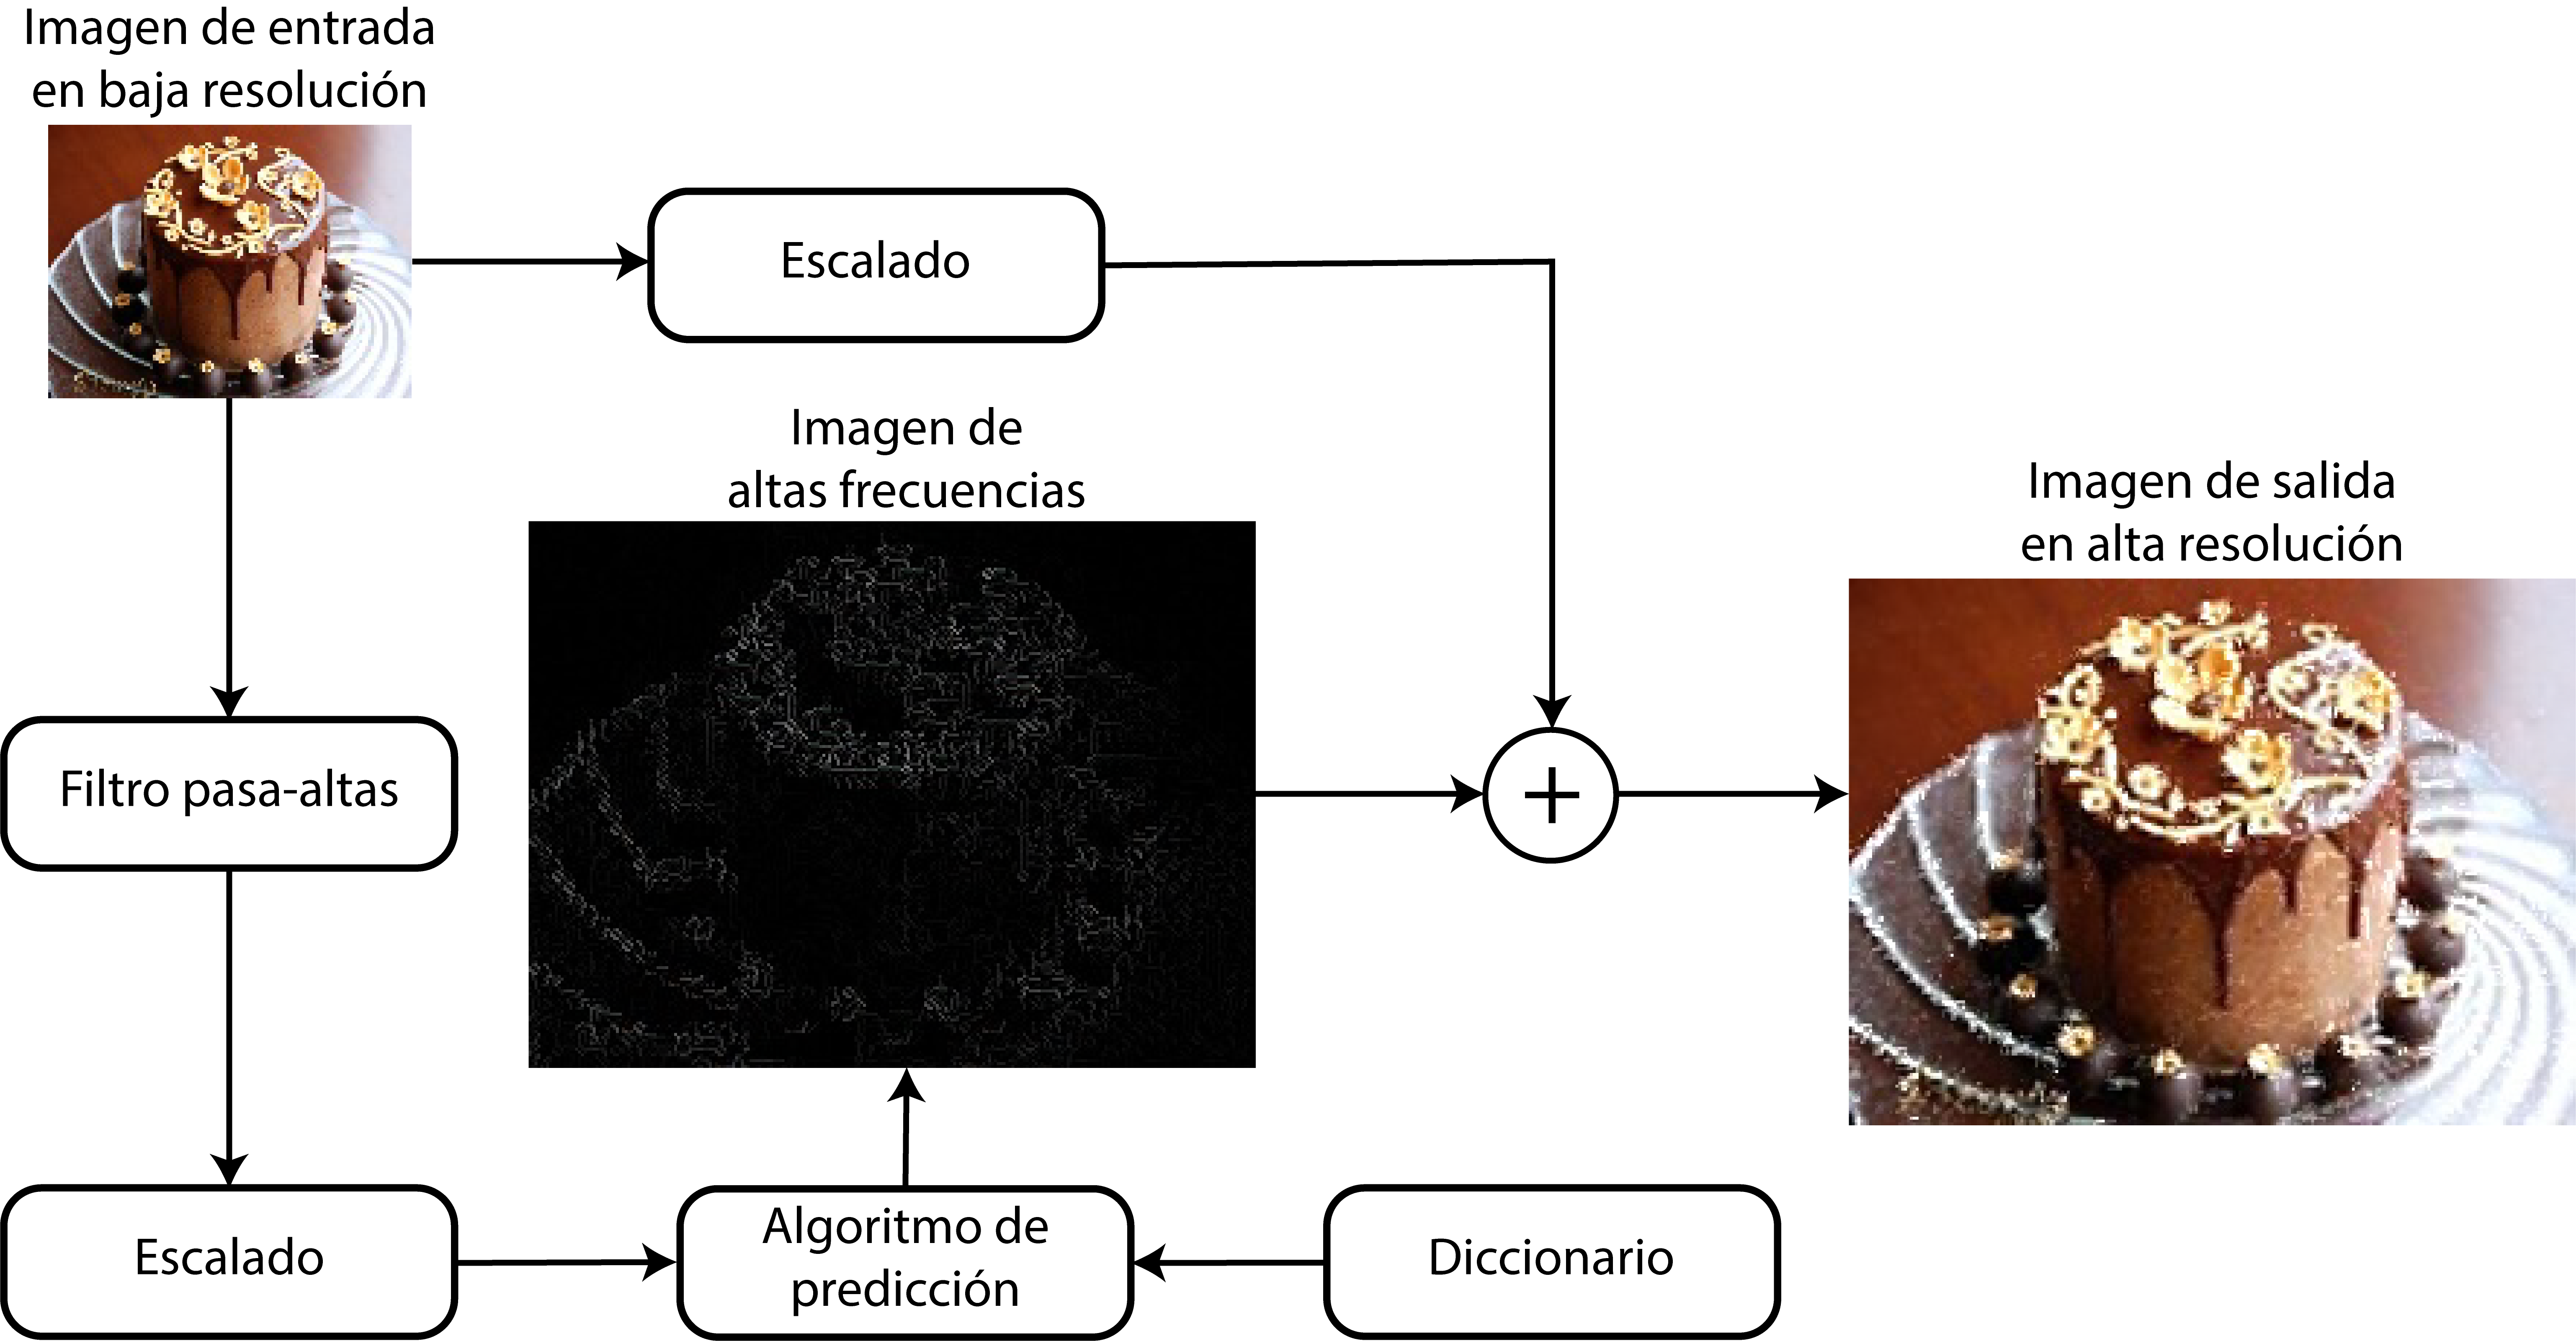
\includegraphics[scale = 0.5]{ fr_proceso.png }
    \centering
    \caption{ Algoritmo de Súper Resolución}
    \label{fig:fr_proceso}
\end{figure}

De igual manera se han realizado variaciones en el factor de superposición
con el objetivo de encontrar el óptimo. En la Figura \ref{fig:fr_alphas}
se presentan algunos de los valores utilizados. 

\begin{figure}[H]
    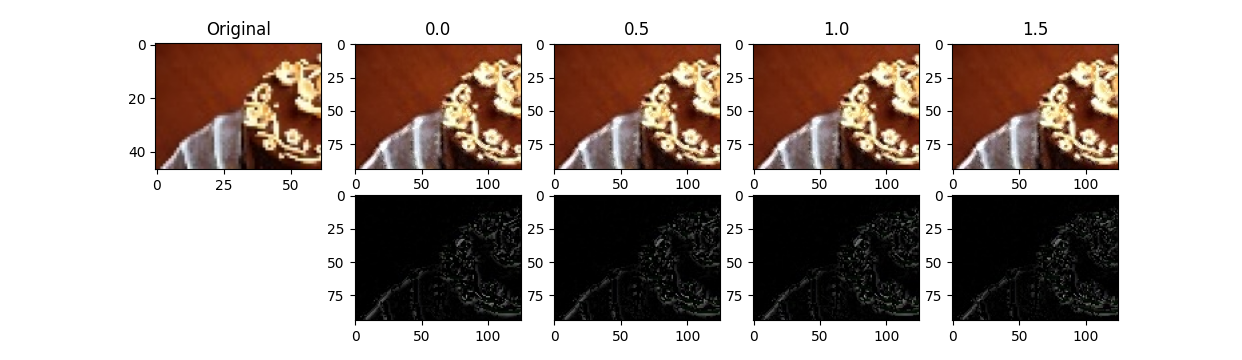
\includegraphics[scale = 0.4]{ fr_alphas.png }
    \centering
    \caption{ Variación en parámetro de superposición $\alpha$ }
    \label{fig:fr_alphas}
\end{figure}

Observe que el parámetro de superposición permite enfatizar los detalles de
la imagen de altas frecuencias e indirectamente los detalles de la
imagen con mejor resolución. 

